%! Author = bvr
%! Date = 2025-03-26

% Preamble
\documentclass[11pt]{article}

% Packages
\usepackage{amsmath}
\usepackage{blindtext}
\usepackage{titlesec}
\usepackage{listings}
\usepackage{graphicx}
\usepackage[T1]{fontenc}

\title{Mnożenie macierzy z wykorzystaniem biblioteki PCJ oraz wątków JVM}
\author{Szymon Orzechowski}
\date{}
\lstset{breaklines=true}
% Document
\begin{document}

    \maketitle

    \clearpage

    \tableofcontents

    \clearpage

    \section{Wstęp}

    Niniejsza praca opisuje rozwiązanie problemu mnożenia macierzy kwadratowych o rozmiarach NxN z wykorzystaniem metod i algorytmów równoległych.
    Projekt został napisany w jezyku Java w wersji 11 z użyciem biblioteki PCJ. W ramach generowania przykładowych danych został przygotowany skrypt
    w języku Python. Program z góry zakłada, że dane dostarczone są poprawne.
    Cały kod źródłowy dostępny jest pod adresem https://github.com/szymonorz/parallel-matrix-multiplier.
    Wideoprezentacja z działania programu i przeglądu kodu znajduje się pod adresem https://www.youtube.com/watch?v=sLUT1OtxHwc.
    
    \section{Specyfikacja oraz instrukcja}

    \subsection{Specyfikacja}
    Specyfikacja środowiska w jakim program był tworzony i testowany wygląda następująco:

    \begin{description}
        \item[System operacyjny] Void Linux (kernel 6.9.12\_1)
        \item[Java] OpenJDK 11
        \item[Python] 3.13.1
        \item[CPU] AMD Ryzen 9 7940HS
    \end{description}

    \subsection{Instrukcja}
    \subsubsection{Przygotowanie danych}

    Został przygotowany skrypt \verb|scripts/helper.py|. Aby wygenerować macierz o rozmiarze \verb|N| pod ścieżką \verb|path| należy wykonać polecenie
    \begin{lstlisting}
        python3 script/helper.py --generate path --size N
    \end{lstlisting}

    Rezultatem tego jest plik o następującym formacie
    \begin{lstlisting}
        N
        a[0][0] a[0][1] ... a[0][N]
        ...
        ...
        a[N][0] a[N][1] ... a[N][N]
    \end{lstlisting}
    gdzie
    \begin{description}
        \item Pierwsza linijka zawiera informację o ilości kolumn i wierszy macierzy
        \item Następne \verb|N| wierszy zawiera po \verb|N| liczb całkowitych z przedziału od 0 do 9
    \end{description}


    \subsubsection{Kompilacja}
    W projekcie został załączony Maven Wrapper oraz dostarczony skrypt \verb|mvnw|. Kompilację należy wykonać poprzez polecenie \verb|./mvnw clean package|.
    Został zastosowany Maven Shade Plugin, którego zadaniem jest zapakowanie wszystkich zależności (takich jak np.: biblioteka PCJ) do pliku JAR
    wraz z programem.

    \subsubsection{Uruchomienie - Tryb PCJ}
    Tryb PCJ jest uruchamiany poprzez wykorzystanie flagi \verb|-p|. Przemnożenie dwóch macierzy pod ścieżkami \verb|matrix1| i \verb|matrix2| oraz zapisanie ich
    w \verb|result-matrix| należy wykonać poniższym poleceniem.

    \begin{lstlisting}
        java -jar target/parallel-....jar --source matrix1 matrix2 --destination result-matrix -p
    \end{lstlisting}

    Wykonanie programu zaskutkuje tym, że zostanie utworzonych \verb|NxN| plik o nazwie, która jest zgodna z formatem \verb|result-matrix.part-{row}-{col}|.
    Owe pliki przechowują wartość komórki macierzy wynikowej \verb|C| w wierszu \verb|row| i kolumnie \verb|col|.

    Scalenie takich komórek należy wykonać poprzez skrypt pomocniczy.

    \begin{lstlisting}
        python3 scripts/helper.py --concat result-matrix
    \end{lstlisting}

    \subsubsection{Uruchomienie - Tryb z wątkami JVM}

    Tryb z użyciem wątków JVM uruchamiamy poprzez flagę \verb|-t|. Tak jak w poprzednim przypadku należy dostarczyć macierze źródłowe i ścieżkę docelową.
    Dodatkowo istnieje opcja ustalenia liczby wątków poprzez flagę \verb|N|. Domyslnie jeżeli nie podamy wartości to program wykona się na jednym wątku.
    \begin{lstlisting}
        java -jar parallel-....jar --source matrix1 matrix2 --destination result-matrix -t -N threadsCount
    \end{lstlisting}

    Po zakończeniu nie ma potrzeby wykonywania operacji scalenia.
    
    \section{Algorytm Cannona - PCJ}

    Niech $A = [a_{ij}]_{N\times N}$ oraz $B = [b_{ij}]_{N\times N}$. Tworzymy siatkę procesów $P$ o rozmiarze $\sqrt{p}\times\sqrt{p}$, gdzie $p$ - ilość procesów.
    Macierze $A, B$ partycjonujemy na $p$ równych kwadratowych podmacieży o rozmiarach $(N/\sqrt{p})\times (N/\sqrt{p})$.
    Kazdy proces $P_{ij}$ z przechowuję dedykowane mu podmacieże $A_{ij}, B_{ij}$.

    Algorytm Cannona dzieli się na następujące kroki:
    \begin{enumerate}
        \item Przesuń i-tą podmacież $A_{ij}$ do procesu $(i, (j-i+\sqrt(p) mod \sqrt(p)))$
        \item Przesuń j-tą podmacież $B_{ij}$ do precesu $((i-j+\sqrt(p)) mod \sqrt(p), j)$.
        \item Na każdym procesie $P_{ij}$ oblicz $C_{ij}$.
        \item Prześlij macierz $A_{ij}$ o 1 w lewo.
        \item Prześlij macierz $B_{ij}$ o 1 do góry.
        \item Wykonuj krok od 3 do 5 $N$ razy.
    \end{enumerate}

    W przypadku algorytmu Cannona każda podmacież $C_i,j$ jest obliczana przez proces $P_i,j$ zgodnie ze wzorem.

    \[C_{ij} = C_{ij} + (A_{ij} * B_{ij})\]

    W przypadku korzystania z bilbioteki PCJ każdy proces $P_{ij}$ zczytuje z plików żródłowych podmacierz o rozmiarach $\sqrt{p}\times\sqrt{p}$
    i następnie podczas przesunięc przesyła oraz odbiera dane między sąsiadującymi procesami. Macierze są trzymane w zmiennych \verb|A_local| oraz \verb|B_local|
    i przesyłane przez \verb|PCJ.put| do sąsiadujących na lewo i górą procesów. Wymiana między procesami jest możliwa dzięki zdefinowaniu zmiennych \verb|A| i \verb|B|
    jako \verb|Shared|. W kolejnym kroku proces czeka, aż otrzyma dane poprzez \verb|PCJ.waitFor()|. Zanim zostaną przekopiowane dane ze zmiennych \verb|A,B| do
    \verb|A_local,B_local| program czeka poprzez użycie \verb|PCJ.barrier| aż wszystkie procesy otrzymają swoje dane.

    Ograniczeniem tej implementacji jest to, że macierze źródłowe muszą się dzielić na równe $\sqrt{p}$ podmacierzy kwadratowych.

    Podczas testowania wydajności wygenerowano macierz 2500x2500 (N=2500) i wykonano program na 1, 4, 25 i 100 procesach
    w każdej iteracji wykonania programu. Program był uruchamiany na 25 procesach JVM.

    \begin{table}[h]
        \centering
        \begin{tabular}{|c|c|}
            \hline
            \textbf{Ilość procesóœ} & \textbf{Czas wykonania (ms)} \\
            \hline
            1  & 37439 \\
            4  & 9685 \\
            25  & 5745 \\
            100  & 8472 \\
            \hline
        \end{tabular}
        \caption{Ilość procesów vs Czas wykonania}
    \end{table}

    \begin{figure}
        \centering
        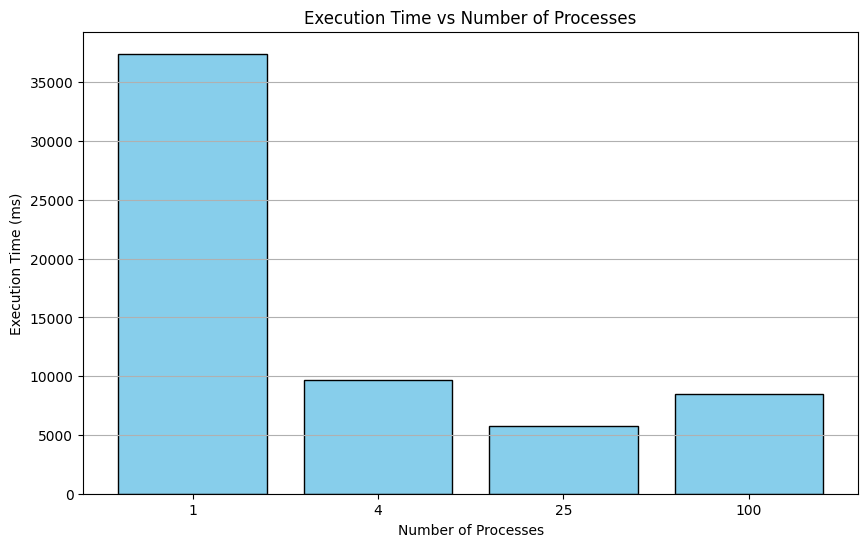
\includegraphics[width=0.8\textwidth]{pcj-plot.png}
        \caption{Wykres czasu wykonania programu w zależności od ilości procesów}
    \end{figure}

    Zwiększony czas wykonania w przypadku 100 procesów wynika głównie z ograniczeń sprzętowych. Urządzenie na którym testowano osiągało limity zużycia CPU i pamięci
    podczas wykonanywania progamu.

    \section{Obliczenie z definicji - wątki JVM}

    W tym trybie mnożenie macierzy następuje zgodnie ze wzorem $wiersz x kolumna$. W ramach podzielenia na wątku wyznaczamy
    dla każdego wątku \verb|startRow| oraz \verb|endRow|, którego przeliczeniem ma się zajmować.

    Podczas testowania wydajności wygenerowano macierz 2500x2500 (N=2500) i wykonano program z inkrementującą się liczbą
    wątków w każdej iteracji wykonania programu.

    \begin{table}[h]
        \centering
        \begin{tabular}{|c|c|}
            \hline
            \textbf{Ilość wątków} & \textbf{Czas wykonania (ms)} \\
            \hline
            1  & 47716 \\
            2  & 21620 \\
            3  & 14376 \\
            4  & 10943 \\
            5  & 8386  \\
            6  & 7114  \\
            7  & 6181  \\
            8  & 5306  \\
            9  & 7534  \\
            10 & 6745  \\
            \hline
        \end{tabular}
        \caption{Ilość wątków vs Czas wykonania}
    \end{table}

    \begin{figure}
        \centering
        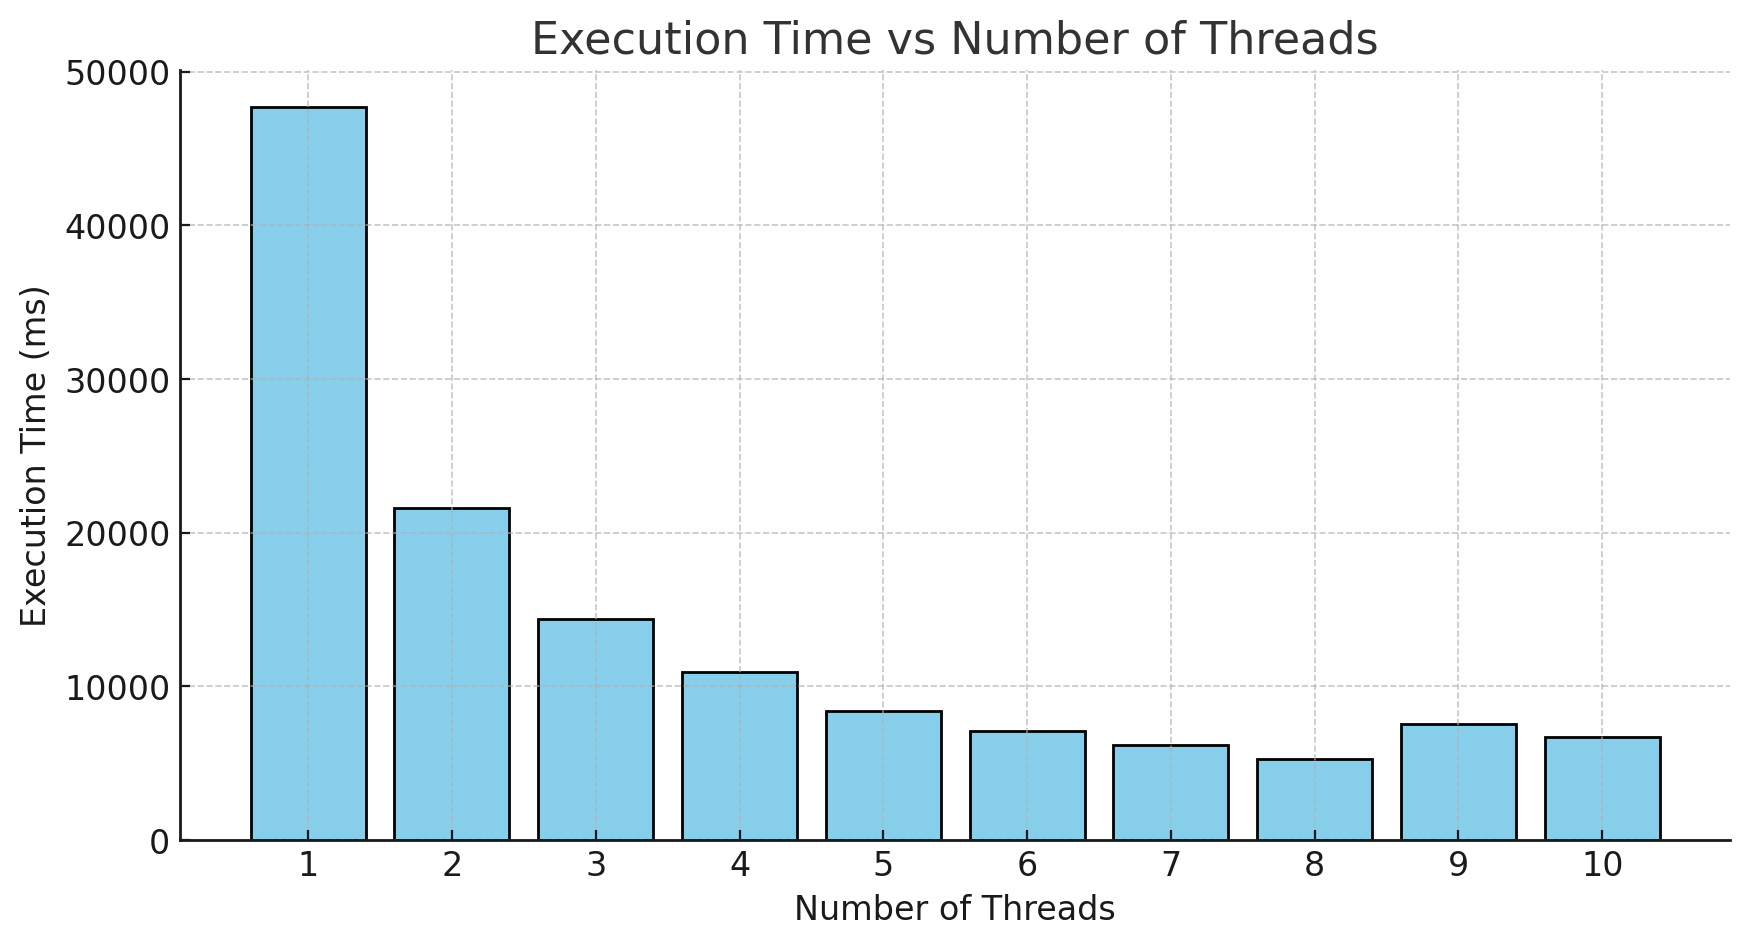
\includegraphics[width=0.8\textwidth]{threads-plot.png}
        \caption{Wykres czasu wykonania programu w zależności od ilości wątków}
    \end{figure}

    Można zauważyć, że wraz z wzrostem ilości wątków czas wykonania maleje lecz już po dojściu do 6 wątków różnice w czasie
    stają się znikome i w niektórych przypadkach czas jest dłuższy niż na mniejszej ilości wątków.

    \clearpage

    \section{Źródła}
    \begin{enumerate}
        \item https://www3.nd.edu/~zxu2/acms60212-40212-S12/Lec-07-3.pdf
    \end{enumerate}
\end{document}